\documentclass[../../../main]{subfiles}
\begin{document}
\subsubsection{Quadrature Encoder}
\label{sub:Theory}
\todo{Bare "in order", ikke first}
\todo{Hvis det her afsnit ligger i design så "ved" vi ikke endnu at det kører på FPGA, dermed lidt hammer intro}
First, in order to understand the implementation of the Quadrature Decoder on the FPGA, a small explanation of how a Quadrature Encoder works is needed. \\
A Quadrature Encoder uses two channels to sense the \todo{Vel også retning?}position of, typically, a rotating disk/shaft or a linear strip. The disk or strip has two paths on it, positioned 90 degresse out of phase with each other, see figure \ref{rotary_encoder} for a rotary encoder and figure \ref{channels_1} for a strip encoder. \todo{Placeres sensorere oven pp encoder eller er det en del af den færdige encoder?}Statinoary sensores are typically placed on top of the encoder, so when a track moves in relation to a sensor, it outputs a logic high or low output signal depending on what part of the track is visible to the sensor. An encoder has two output signals, one for each channel, typically called A and B, see figure \ref{channels_1} for a representation of those for both encoder types. This two signals, A and B, is what \todo{allows the encoder to determine the position and direction of the encoder}the decoder uses to determine the position of the encoder.

\begin{figure}[H]
  
\includegraphics[width = \textwidth]{\main/afsnit/system_implementation/Quadraturdecoder/pictures/encoder.png}
  \caption{Tracks of a rotary encoder.}
  \label{rotary_encoder}
\end{figure}
\todo{Blå overskrifter skriger bare WORD 2010 :D}

\begin{figure}[H]
  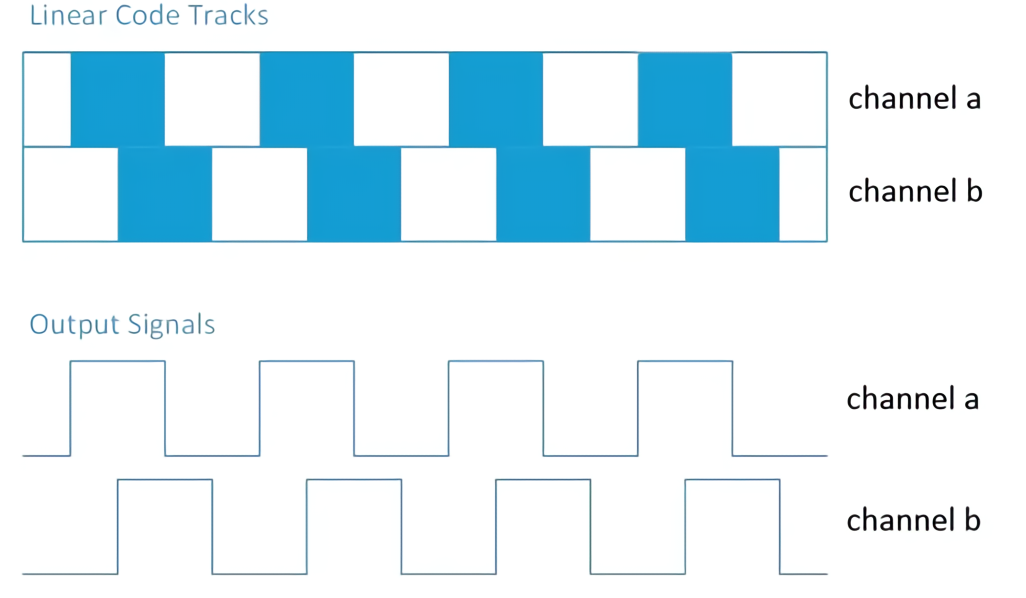
\includegraphics[width = \textwidth]{\main/afsnit/system_implementation/Quadraturdecoder/pictures/channels.png}
  \caption{The upper figure a Linear encoder and the lower figure shows the logic output of both a rotary and linary encoder}
  \label{channels_1}
\end{figure}

\subsubsection{Decoder principle}
The \todo{Founding principle of a Quadratur decoder relies on decoding the relationship between the two outputs and deduce a position change}basic principle of a Quadrature Decoder is for it to decode the two output signals the encoder produces and return a position. The idea is to observe both encoder outputs. By counting the transitions from high to low and low to high on just one of the outputs, it can be determined how far the encoder has rotated. However, by adding the second output, the direction of the encoder can be computed as well as \todo{increasing the resolution}adding a higher resolution to the position. The encoder used in the project is a rotary encoder with a resolution of 360\footnote{See datasheet x}, which means that the Quadrature Decoder will count 360 "ticks" per shaft turn. This resolution and rotation can not be mapped directly to the system itself as its motors are geared. The motors do three full rotations of their shafts before the system itself has completed a full rotation. Hence the resolution for the system is \todo{ticks}1080. This is very useful, since it gives a $\frac{1}{3}$ of a degrees position precision.
\subsubsection{Statemachine}
To use the transitions between encoder output A and output B, a truth table of every possible combination of the two singals must be computed. As mentioned in system design it is necessary to include a third signal called \todo{Hedder return to home her, men reset i tabel?}"return to home" in order to reset the position counter if a new reference point is desired. The truth table including all three signals is shown in figure \ref{fig:truth_table}.
\begin{figure}[H]
  \begin{tabular}{|c | c | c | c | c | c |c|}
  \hline
   A\_prev & A\_new & B\_prev & B\_new & Reset & Direction & Position \\
   \hline
   0 & 1 & 0 & 0 & 1 & Forward & + 1 \\
   1 & 1 & 0 & 1 & 1 & Forward & + 1 \\
   1 & 0 & 1 & 1 & 1 & Forward & + 1 \\
   0 & 0 & 1 & 0 & 1 & Forward & + 1 \\
   0 & 0 & 0 & 1 & 1 & Backward & - 1 \\
   1 & 0 & 0 & 0 & 1 & Backward & - 1 \\
   0 & 1 & 1 & 1 & 1 & Backward & - 1 \\
   1 & 1 & 1 & 0 & 1 & Backward & - 1 \\
   x & x & x & x & 0 & No change &  0 \\
   \hline
  \end{tabular}
  \caption{This figure shows the truth table for the Quadrature decoder}
  \label{fig:truth_table}
\end{figure}
The truth table shows nine possible scenarios that can occur from tracking the transistions of the outputs. Four of these results in a forward direction and the counter will increment, four scenarios results in a backwards direction and the counter will decrement. The last scenario occurs if the reset flag is set low\footnote{Reset is implemented as active low, as can be observed in the truth table \ref{fig:truth_table}.}, and the counter is set to zero regardless of what it was on before. From these observations a state machine containing 6 states has been computed. The states are: AB\_low with the gray code $001$\footnote{The first digit is signal A, second is signal B and thrid is the reset signal}, AB\_high with gray code $111$, A\_high with gray code $101$, B\_high with gray code $011$, undefined and reset $xx0$. The undefined state is purely for debugging purposes used if an error with the signal A and B ocurs. A potential error could be if the state is currently AB\_low the gray code can not be $111$ in the next instance. This would mean that both signals changed at the same time. The state machine diagram is shown below in figure \ref{state_dia}. \\
The decoder works by first initialalizing and go to a state depending on the level of signal A and B. The decoder will then use the debounced signals to determine the next state. If the starting state is AB\_low, there is three correct outcomes: the reset signal goes low and the counter will go to zero, the signal A goes high and the state changes to A\_high or the last possible outcome, that does not give an error, is B\_high. By looking at the truth table from the above figure \ref{fig:truth_table}, it can be observed that if the state goes from AB\_low to A\_high, the direction will be forward and the counter will increment where the counter would decrement and direction set to backwards if the next state is B\_high.\\
The counter keeps track of the position of the encoder. The counter counts position zero as the angle the system was in, as the encoder was initialized. It is thereforth considered useful to add a reset function, so a new \todo{reference er et uheldigt navn, det hedder det også i PID måske home}reference point can be added as desired.  The Statemachine approach has been implemented and the process described in section \ref{system_implementation}

\begin{figure}[H]
  \centering
  \def\svgwidth{\columnwidth}
  \fontsize{9}{9}\selectfont
  \includesvg[\main/afsnit/system_implementation/Quadraturdecoder/pictures/]{decoder_state}
  \caption{}
\end{figure}
As mentioned above, a reset is needed for the application. This allows for a new \todo{reference igen}reference point to be set as desired. The state machine does not make use of a clock singal so the reset is \todo{required}desired to be a asyncron reset to avoid adding more complications to the application. 
\subsubsection{Velocity measure}
The decoder is not only responsible for computing the position of the system but also the velocity. The simplest way to estimate the velocity is by diving the change in position with the change in time. The most classic options are either to keep the $\Delta$t fixed, measure the position between the interval and then take the difference between x(n) and x(n-1) as shown in equation \ref{eq_1}. The other is to keep the position fixed and compute how long it takes to reach the fixed  $\Delta$x like in equation \ref{eq_2}.
\begin{equation}
v(n) = \frac{x(n)-x(n-1)}{T}
\label{eq_1}
\end{equation}
\begin{equation}
  v(n) = \frac{X}{t(n)-t(n-1)}
  \label{eq_2}
\end{equation}
The second approach \ref{eq_2} is considered the most reliable at slow speeds, which arguably the system does fall under. However, this approach depends on the output to be a "fixed interval pulse train". The system does not fit this criteria, because it generates different frequency waves depending on the supplied PWM value\footnote{https://www.embeddedrelated.com/showarticle/158.php}. 
\\
\\
\todo{Denne sætning er lidt mudret prøv igen ?}
The other approach is not hindred by this, so that one has been chosen
As the first approach using equation \ref{eq_1} is not hindred by the difference in frequency, as long as it does not affect the timer, it has been chosen as the desired appraoach. \\


As this approach requires a fixed interval one such must be decided. The issue to take into account here is to make sure the interval is neither too short or too long. A too short interval might yield scenario where the velocity seems to be zero even if the system does move. However, on the opposite side, a too long interval could yield a scenario that gives a wrong velocity, if the system changes velocity a lot. If the interval is say 1 second, \todo{Forstår hvad du mener men det er mudret}the velocity at the first $10ms$ be 50 ticks, but it slows down considerably at the $20ms$ mark and hardly moves at $70ms$ mark. This will give an average velocity that might not be as useful and downright misleading as it shows the system to have travelled with a low speed instead of a showing that it was fast at first but slow towards the end. In this case it is important to the system speed up and slow down, so a low interval time of $10ms$ has been chosen.

\end{document}
